\section{Evaluation}
\label{sec:evaluation}

%We conducted a comprehensive evaluation of SuffixDecoding to assess its performance from both the perspective of speculation efficacy and overall system performance. In our end-to-end experiments, we compared SuffixDecoding with SpecInfer, which is an existing state-of-the-art framework for LLM serving that utilizes tree-based speculative decoding. We performed detailed ablation studies to highlight the contribution of each component of our technique to the overall performance. This section is organized as follows: Section \ref{sec:evaluation-methodology} outlines the experimental setup, Section \ref{sec:main-experiment-results} presents the results of the experiments and provides an in-depth discussion, and Section \ref{sec:ablation-experiments} details the ablation studies.

\subsection{Evaluation Methodology}
\label{sec:evaluation-methodology}

\begin{wrapfigure}{r}{0.5\textwidth}
\centering
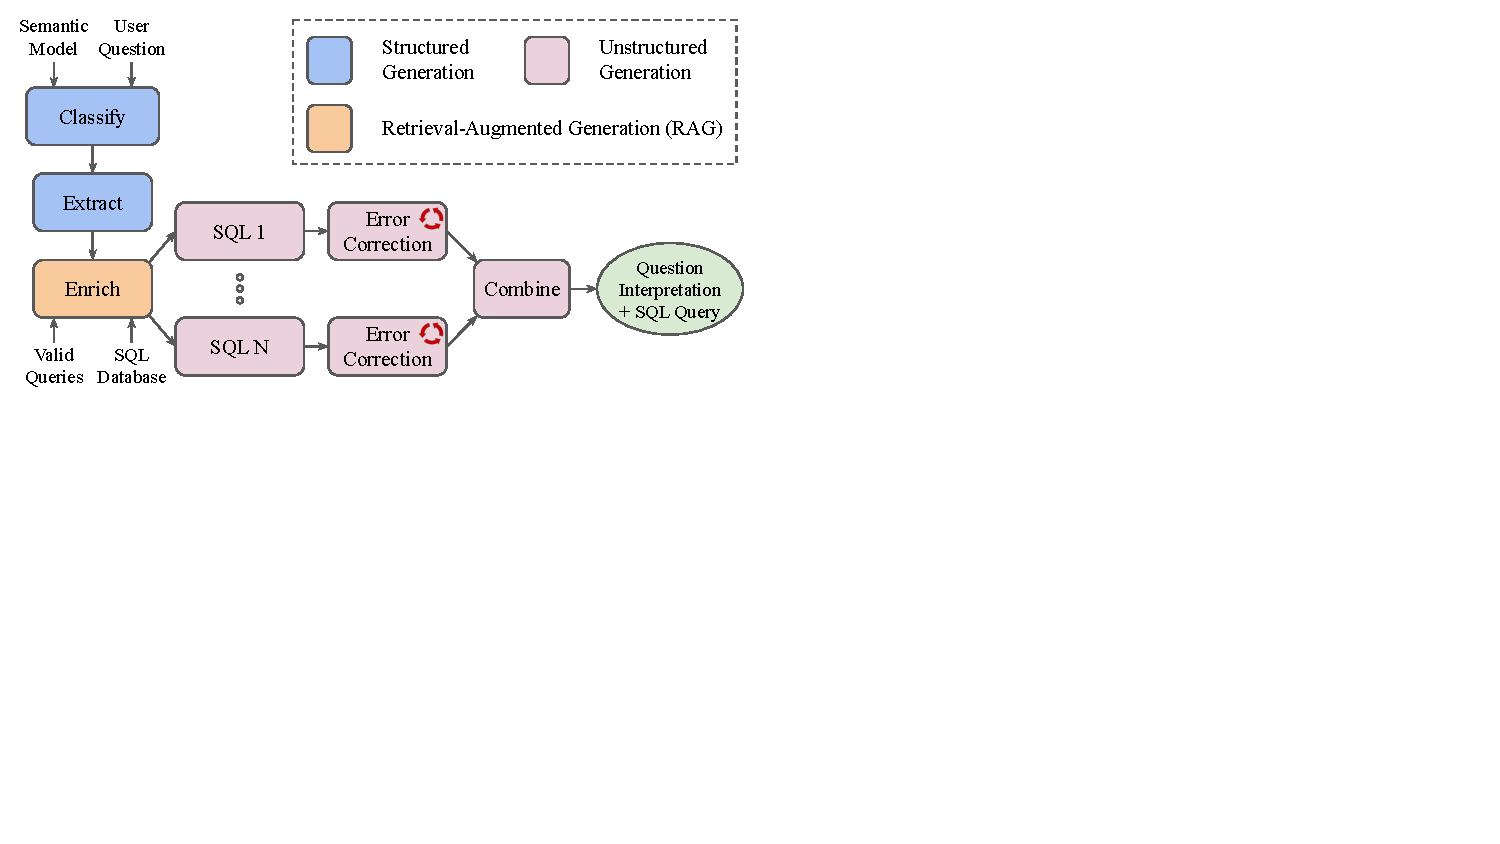
\includegraphics[width=0.5\columnwidth,trim={0 220 360 0},clip]{figures/agentic-sql.pdf}
\caption{AgenticSQL is a multi-agent workflow consisting of stuctured generation, unstructured generation, and retrieval-augmented generation steps across several different LLMs. Useful features are extracted from the user question (Classify and Extract) and supplemented with retrieved context (Enrich). Several text-to-SQL steps propose solutions to the user question (SQL 1\ldots N) in parallel with feedback from an error corrector. A last Combine step synthesizes the proposed SQL candidates into a final SQL query and text response.}
\label{fig:agentic-sql}
\end{wrapfigure}

\paragraph{Baseline Comparisons.}
We compare with both model-based and model-free speculative decoding methods using Spec-Bench~\citep{xia2024unlockingefficiencylargelanguage}. (1) \emph{EAGLE-2} and \emph{EAGLE-3}~\citep{li2025eagle3scalinginferenceacceleration}, state-of-the-art model-based speculators, (2), \emph{Prompt-Lookup Decoding (PLD)}~\citep{saxena2023prompt}, a simple model-free speculator based on ngram-matching, and (3) \emph{Token Recycling}~\citep{luo2024turningtrashtreasureaccelerating}, a more recent model-free speculator that sources token sequences from both the prompt and previous outputs. EAGLE-3 and Token Recycling both leverage tree speculation~\citep{specinfer}.

\paragraph{Datasets and Agentic Applications.}
We evaluate on both agentic and non-agentic workloads. For agentic applications, we trace requests from two real applications: OpenHands~\citep{openhands} on \emph{SWE-Bench}~\citep{jimenez2024swebenchlanguagemodelsresolve} (a GitHub issue resolution benchmark), and \emph{AgenticSQL}, a proprietary multi-agent SQL generation workflow (Fig.~\ref{fig:agentic-sql}). For non-agentic workloads, we use Spec-Bench, consisting of open-ended, single-turn tasks across 13 categories, including 8 MT-Bench categories (Writing, Roleplay, Reasoning, Math, Coding, Extraction, STEM, Humanities). We include Spec-Bench to stress-test SuffixDecoding's limitations and evaluate the hybrid fallback mechanism.

\paragraph{End-to-end System Evaluation.} We implemented SuffixDecoding in vLLM~\citep{kwon2023efficientmemorymanagementlarge}. By running OpenHands live, we show SuffixDecoding accelerates end-to-end task completion times, including prefill and code execution.

\paragraph{Hardware configuration.}
We conducted our experiments on a single \texttt{p5.48xlarge} AWS instance equipped with \( 8\times \) NVIDIA H100 80G GPUs and 2TB of main memory.

\paragraph{Simulated Ablations.}

In addition to our main evaluation using real hardware, we also leverage a simulated verifier for additional experiments in Sec.~\ref{sec:ablation-experiments} and continued in Appendix~\ref{sec:additional-ablation-experiments}. Given a prompt \( x_{1:n} \) and example ground-truth response \( y_{n+1:t} \), we can accurately simulate speculative verification for greedy sampling by verifying that speculated token \( x_{n+i} = y_{n+i} \).

\subsection{Baseline Comparisons}
\label{sec:baseline-comparisons}
\begin{figure*}
\centering
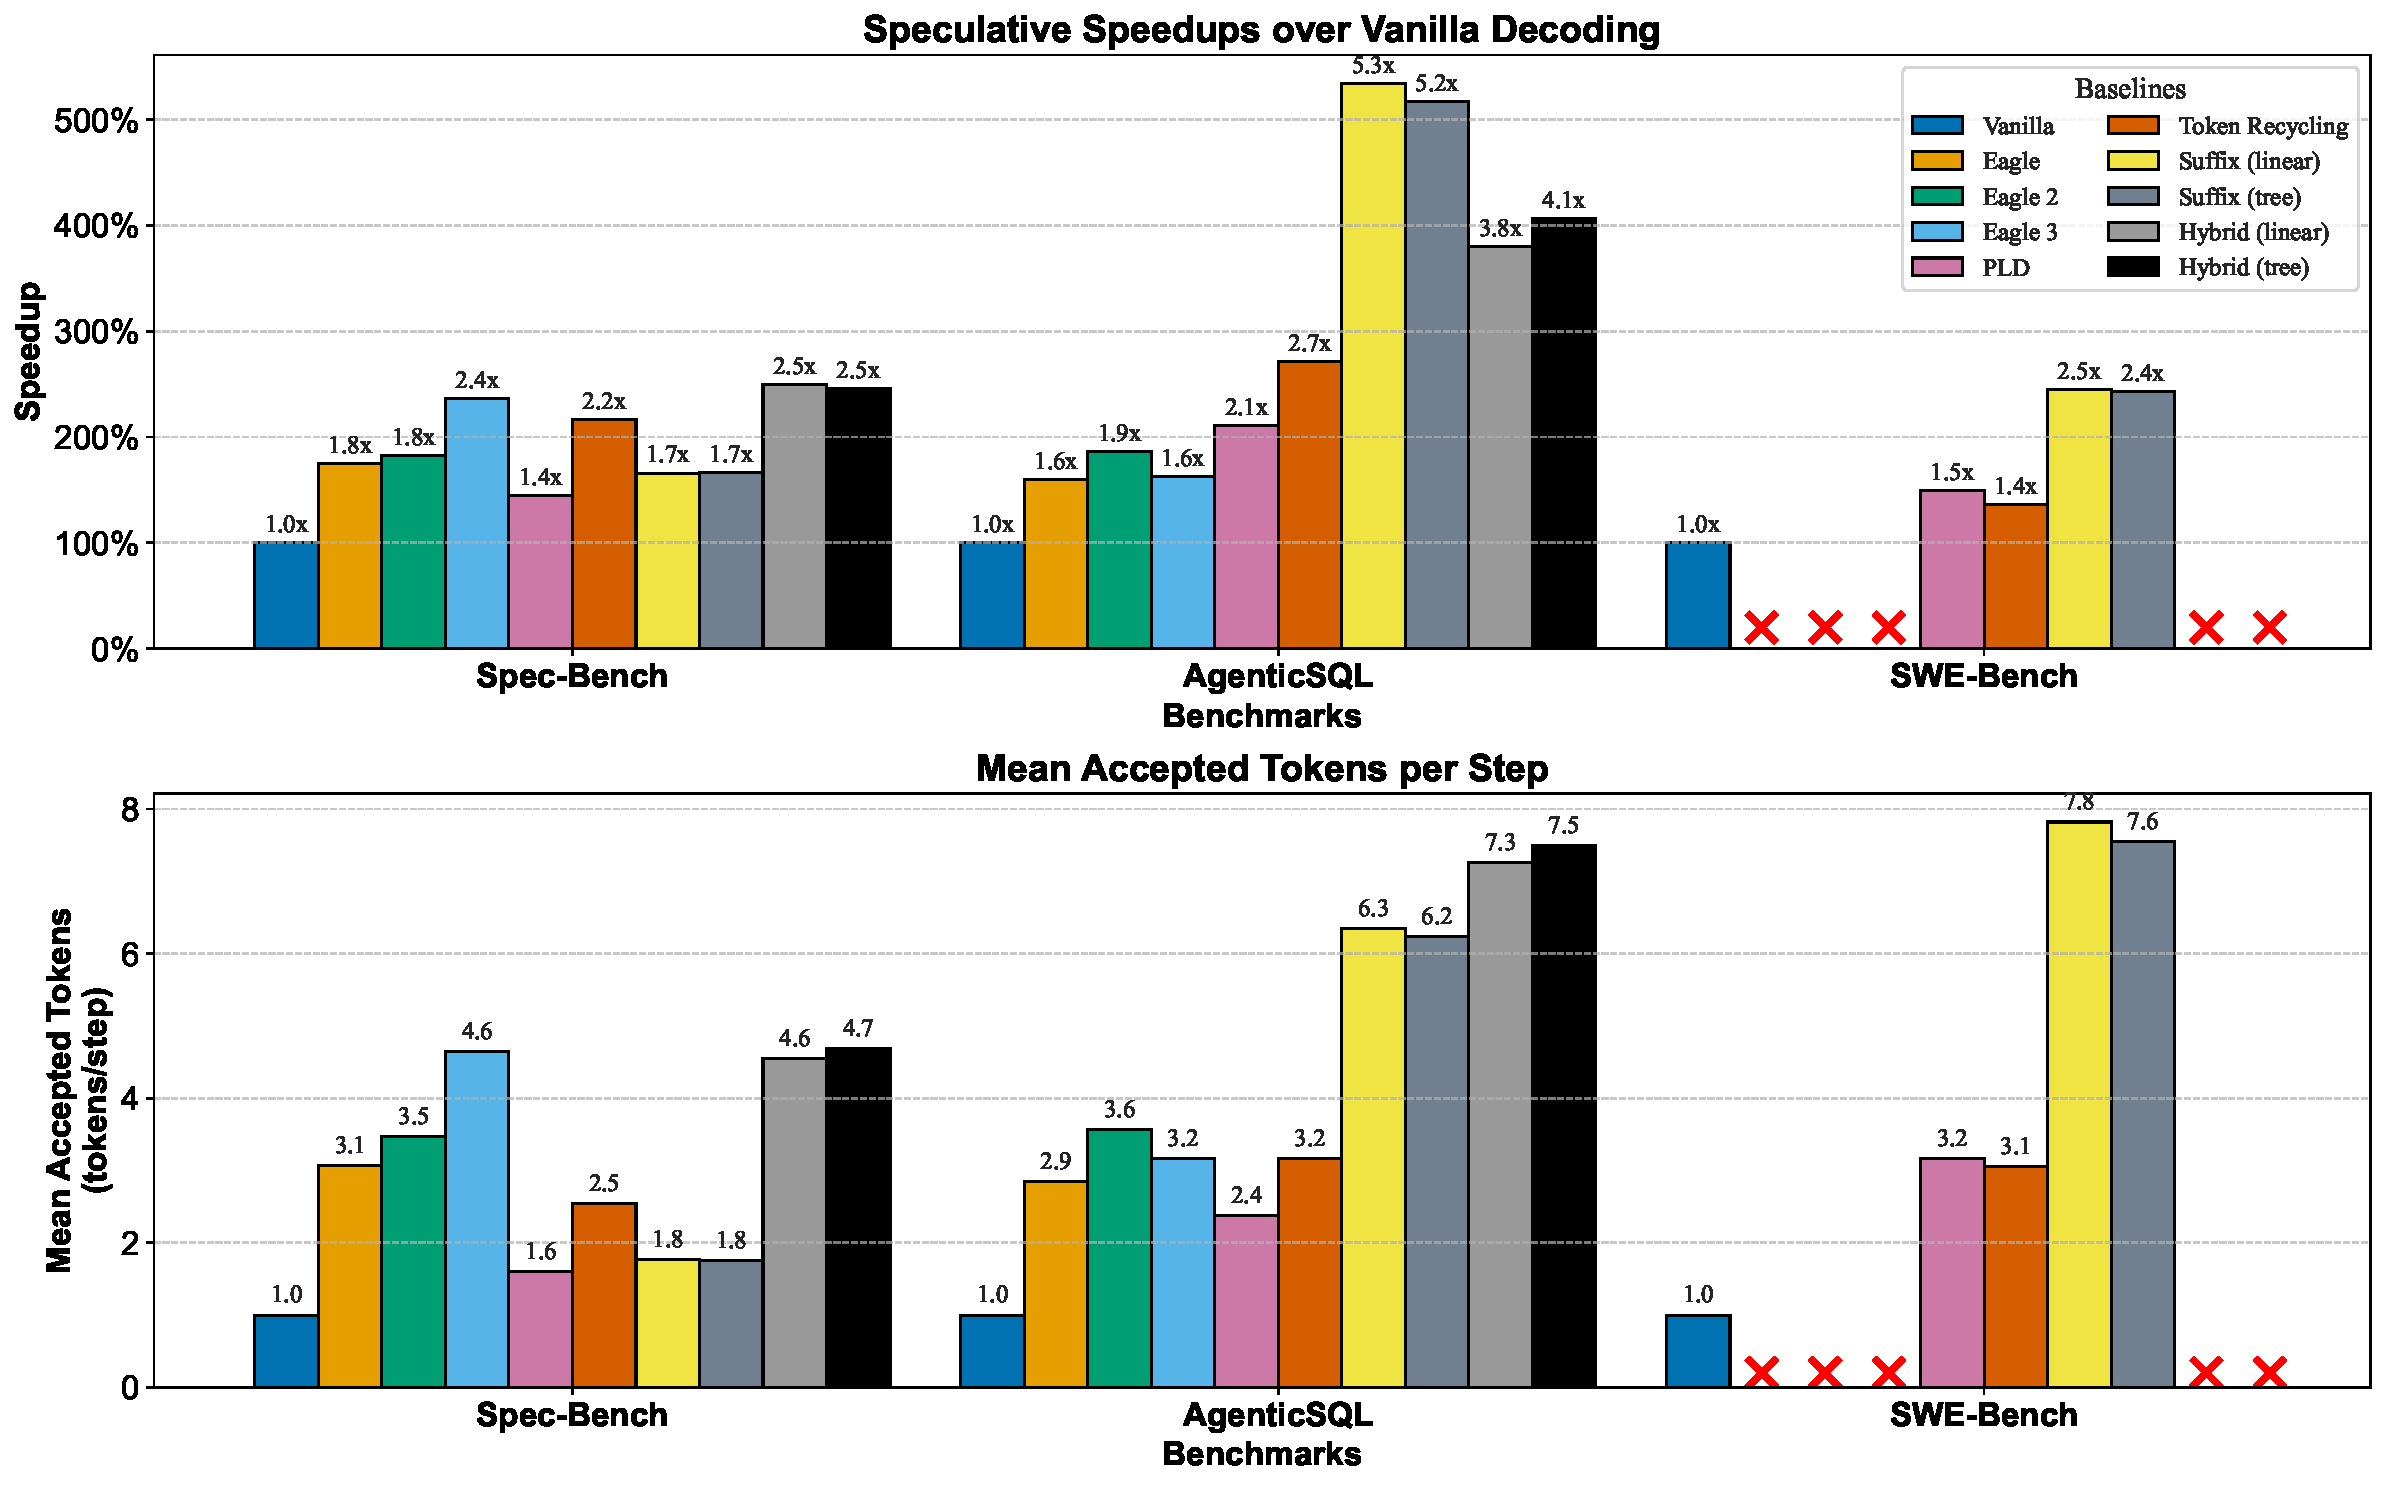
\includegraphics[width=\linewidth]{latex/figures/benchmark_comparison.pdf}
\caption{Speculative speedups (top) and mean accepted tokens per step (bottom) compared to vanilla decoding for SuffixDecoding and baseline methods on three benchmarks: Spec-Bench, AgenticSQL, and SWE-Bench. Experiments use Llama-3.1-8B-Instruct on a single H100 GPU with batch size 1. Speedup is measured as the ratio of wall-clock time-per-output-token relative to vanilla decoding. Suffix (tree) and Hybrid (tree) use SuffixDecoding's tree speculation algorithm, which constructs a speculation tree from the suffix tree for parallel verification. Suffix (linear) and Hybrid (linear) use a simpler linear speculation approach that only allows sequential token chains. The hybrid variants combine SuffixDecoding with EAGLE-3, dynamically selecting between suffix-based and model-based speculation based on pattern match confidence. Note that EAGLE-2/3 and Token Recycling failed to run on several SWE-Bench tasks due to long context lengths (>8192 tokens), indicated by missing bars. Spec-Bench represents a non-agentic workload and is included for comparison. Further sub-task breakdowns, including the raw time-per-output-token and mean acceptance lengths, can be found in Appendix~\ref{sec:main-experiment-details}.}
\label{fig:throughput-tpot}
\end{figure*}



We compare SuffixDecoding with EAGLE-2, EAGLE-3, PLD, and Token Recycling on SWE-Bench and AgenticSQL. We also run the Spec-Bench standard dataset, which is a more traditional non-agentic workload. Fig.~\ref{fig:throughput-tpot} shows the results. First, on the agentic workloads, SuffixDecoding outperforms all baselines. In AgenticSQL, SuffixDecoding obtains a mean speedup of $5.3\times$ over vanilla decoding, a $2.8 \times$ improvement over EAGLE-2/3, and $1.9\times$ higher than Token Recycling. In SWE-Bench, EAGLE-2/3 fail due to their maximum sequence length limitations. SuffixDecoding obtains a mean speedup of $2.5\times$ over vanilla decoding, a $1.7 \times$ improvement over PLD, the next best baseline. SuffixDecoding’s superior performance in agentic workloads can be attributed to its consistently higher mean accepted tokens per decoding step. In AgenticSQL, SuffixDecoding reaches 6.3 mean accepted tokens per step—substantially higher than EAGLE-3 (3.6 tokens) and Token Recycling (3.2 tokens). In SWE-Bench, SuffixDecoding achieves 7.8 mean accepted tokens per step, while PLD only accepts 3.2 tokens per step on average.

On non-agentic workloads such as Spec-Bench (which includes open-ended single-turn tasks and 8 MT-Bench categories), SuffixDecoding alone is outperformed by EAGLE-2/3 and Token Recycling, as expected for less repetitive scenarios. However, the hybrid approach of SuffixDecoding + EAGLE-3 achieves the best of both worlds: we speculate with the faster SuffixDecoding method whenever possible and fall back to EAGLE-3 when the speculation score is too low. The Hybrid approach obtains a mean speedup of $2.5\times$ over vanilla decoding, outperforming the $2.4\times$ speedup from standalone EAGLE-3 and the $2.2\times$ speedup from Token Recycling.

The hybrid approach also performs well in AgenticSQL, achieving a $4.1\times$ speedup in the tree variant, significantly better than the $1.9\times$ speedup from standalone EAGLE-2/3 and the $2.7\times$ speedup from Token Recycling. These speedups are achieved thanks to the hybrid approach's impressive 7.5 mean accepted tokens per step, more than $2\times$ higher than EAGLE-2/3 and Token Recycling. SuffixDecoding has a slightly lower mean acceptance length of 6.3, but its much lower speculation cost and higher acceptance rate make it the winning solution in agentic tasks ($5.3\times$ average speedup compared to the $4.1\times$ speedup of the hybrid approach). 

\paragraph{A peek into a speculation tree. }

\begin{wrapfigure}{R}{0.6\textwidth}
    \centering
    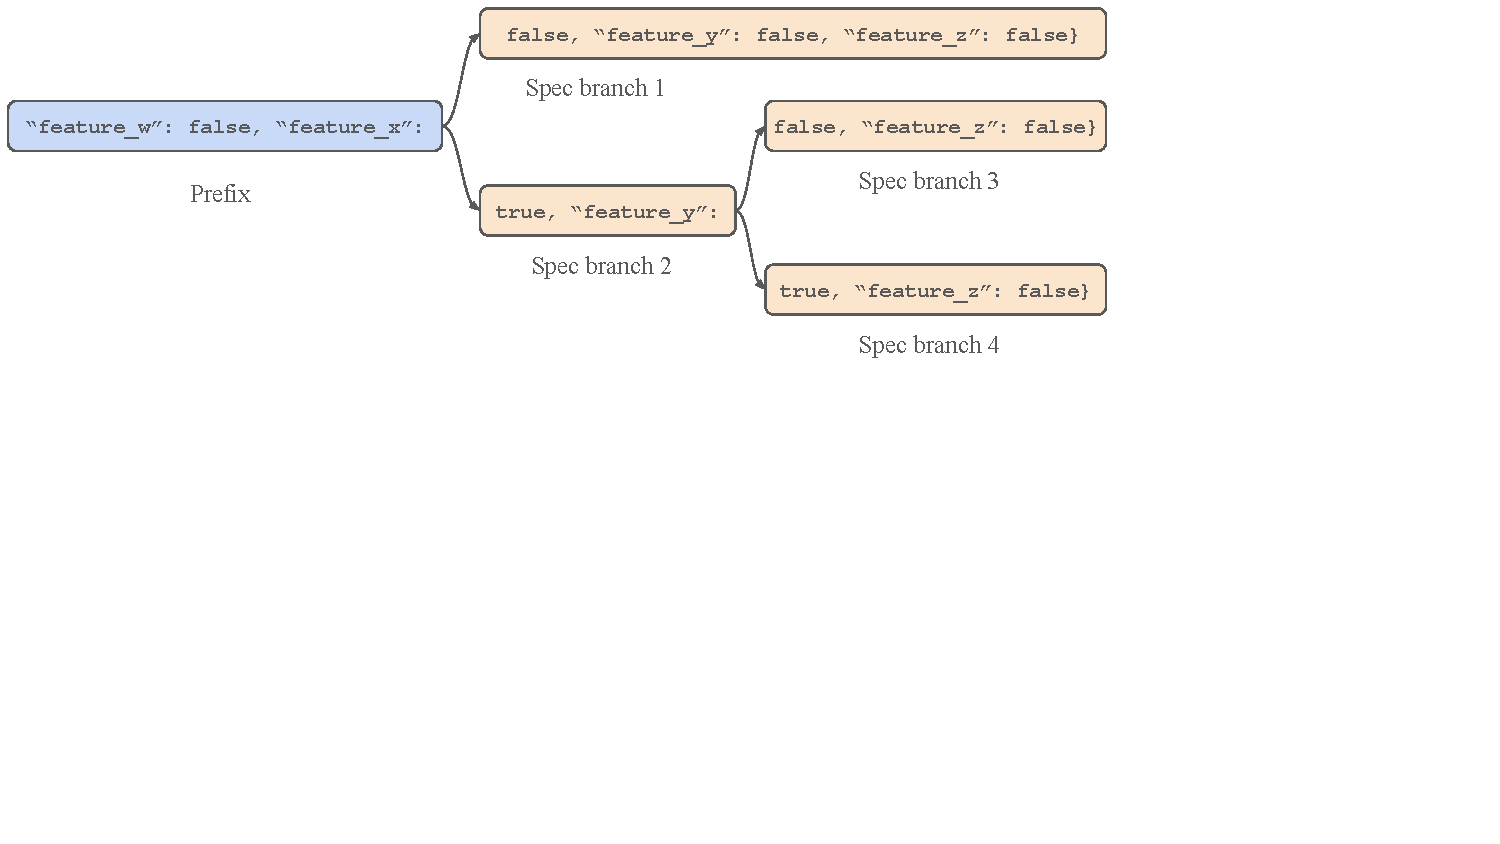
\includegraphics[width=0.6\columnwidth,trim={0 230 180 0},clip]{figures/speculation-tree-example.pdf}
    \caption{A SuffixDecoding speculation tree containing 66 tokens for the AgenticSQL Extract task.}
    \label{fig:speculation-tree-example}
\end{wrapfigure}

To gain some intuition into why SuffixDecoding performs so well for certain tasks, we examine how it builds a speculation tree for the AgenticSQL Extract task.
The outputs of the Extract task have many characteristics in common. First, they are all JSON documents following the same format and key names, with keys often appearing in the same order. Second, many of the features are discrete values, and in particular, boolean true/false values. These patterns are recorded in SuffixDecoding's global suffix tree and guide its speculation tree construction.

Fig.~\ref{fig:speculation-tree-example} shows an example of a speculation tree constructed by SuffixDecoding. We observed many instances of large speculation trees that branch at each boolean true/false value of several consecutive features. These speculation tree always contains a branch with high acceptance, advancing output generation by dozens of tokens or more in one step. 
Although this is one specific example of a speculation tree, it demonstrates that SuffixDecoding can find complex patterns in previous outputs, particularly for structured generation tasks, that help accelerate output generation.

\subsection{End-to-End SWE-Bench on vLLM}
\label{sec:vllm-swebench-results}

In this section, we show that SuffixDecoding can be efficiently integrated into vLLM, a popular inference system used in production deployments, and it can effectively accelerate accelerate end-to-end agentic task completion time. For this experiment, we run OpenHands directly on vLLM with SuffixDecoding, so the agent is solving each benchmark problem live. We also use the specially-trained LLM \texttt{all-hands/openhands-lm-32b-v0.1-ep3}, which was fine-tuned for SWE-Bench and achieves 37.2\% on SWE-Bench Verified. Since there are no model-based methods with draft models trained for this LLM, we compare with vLLM's native implementation of PLD. 

Fig.~\ref{fig:vllm-spec-bench} shows the results. First, we note that decoding time (i.e. output generation) takes a majority of the time across all SWE-Bench tasks, dominating both prefilling and agentic actions (i.e. code execution). In this end-to-end scenario, SuffixDecoding outperforms PLD by 1.3--3\(\times\), leading to a 1.8--4.5\(\times\) speculative speedup over vanilla decoding. Since SuffixDecoding exactly preserves the output distribution of the LLM, it matches the original model's 37.2\% score on SWE-Bench Verified.

\begin{figure}
\centering
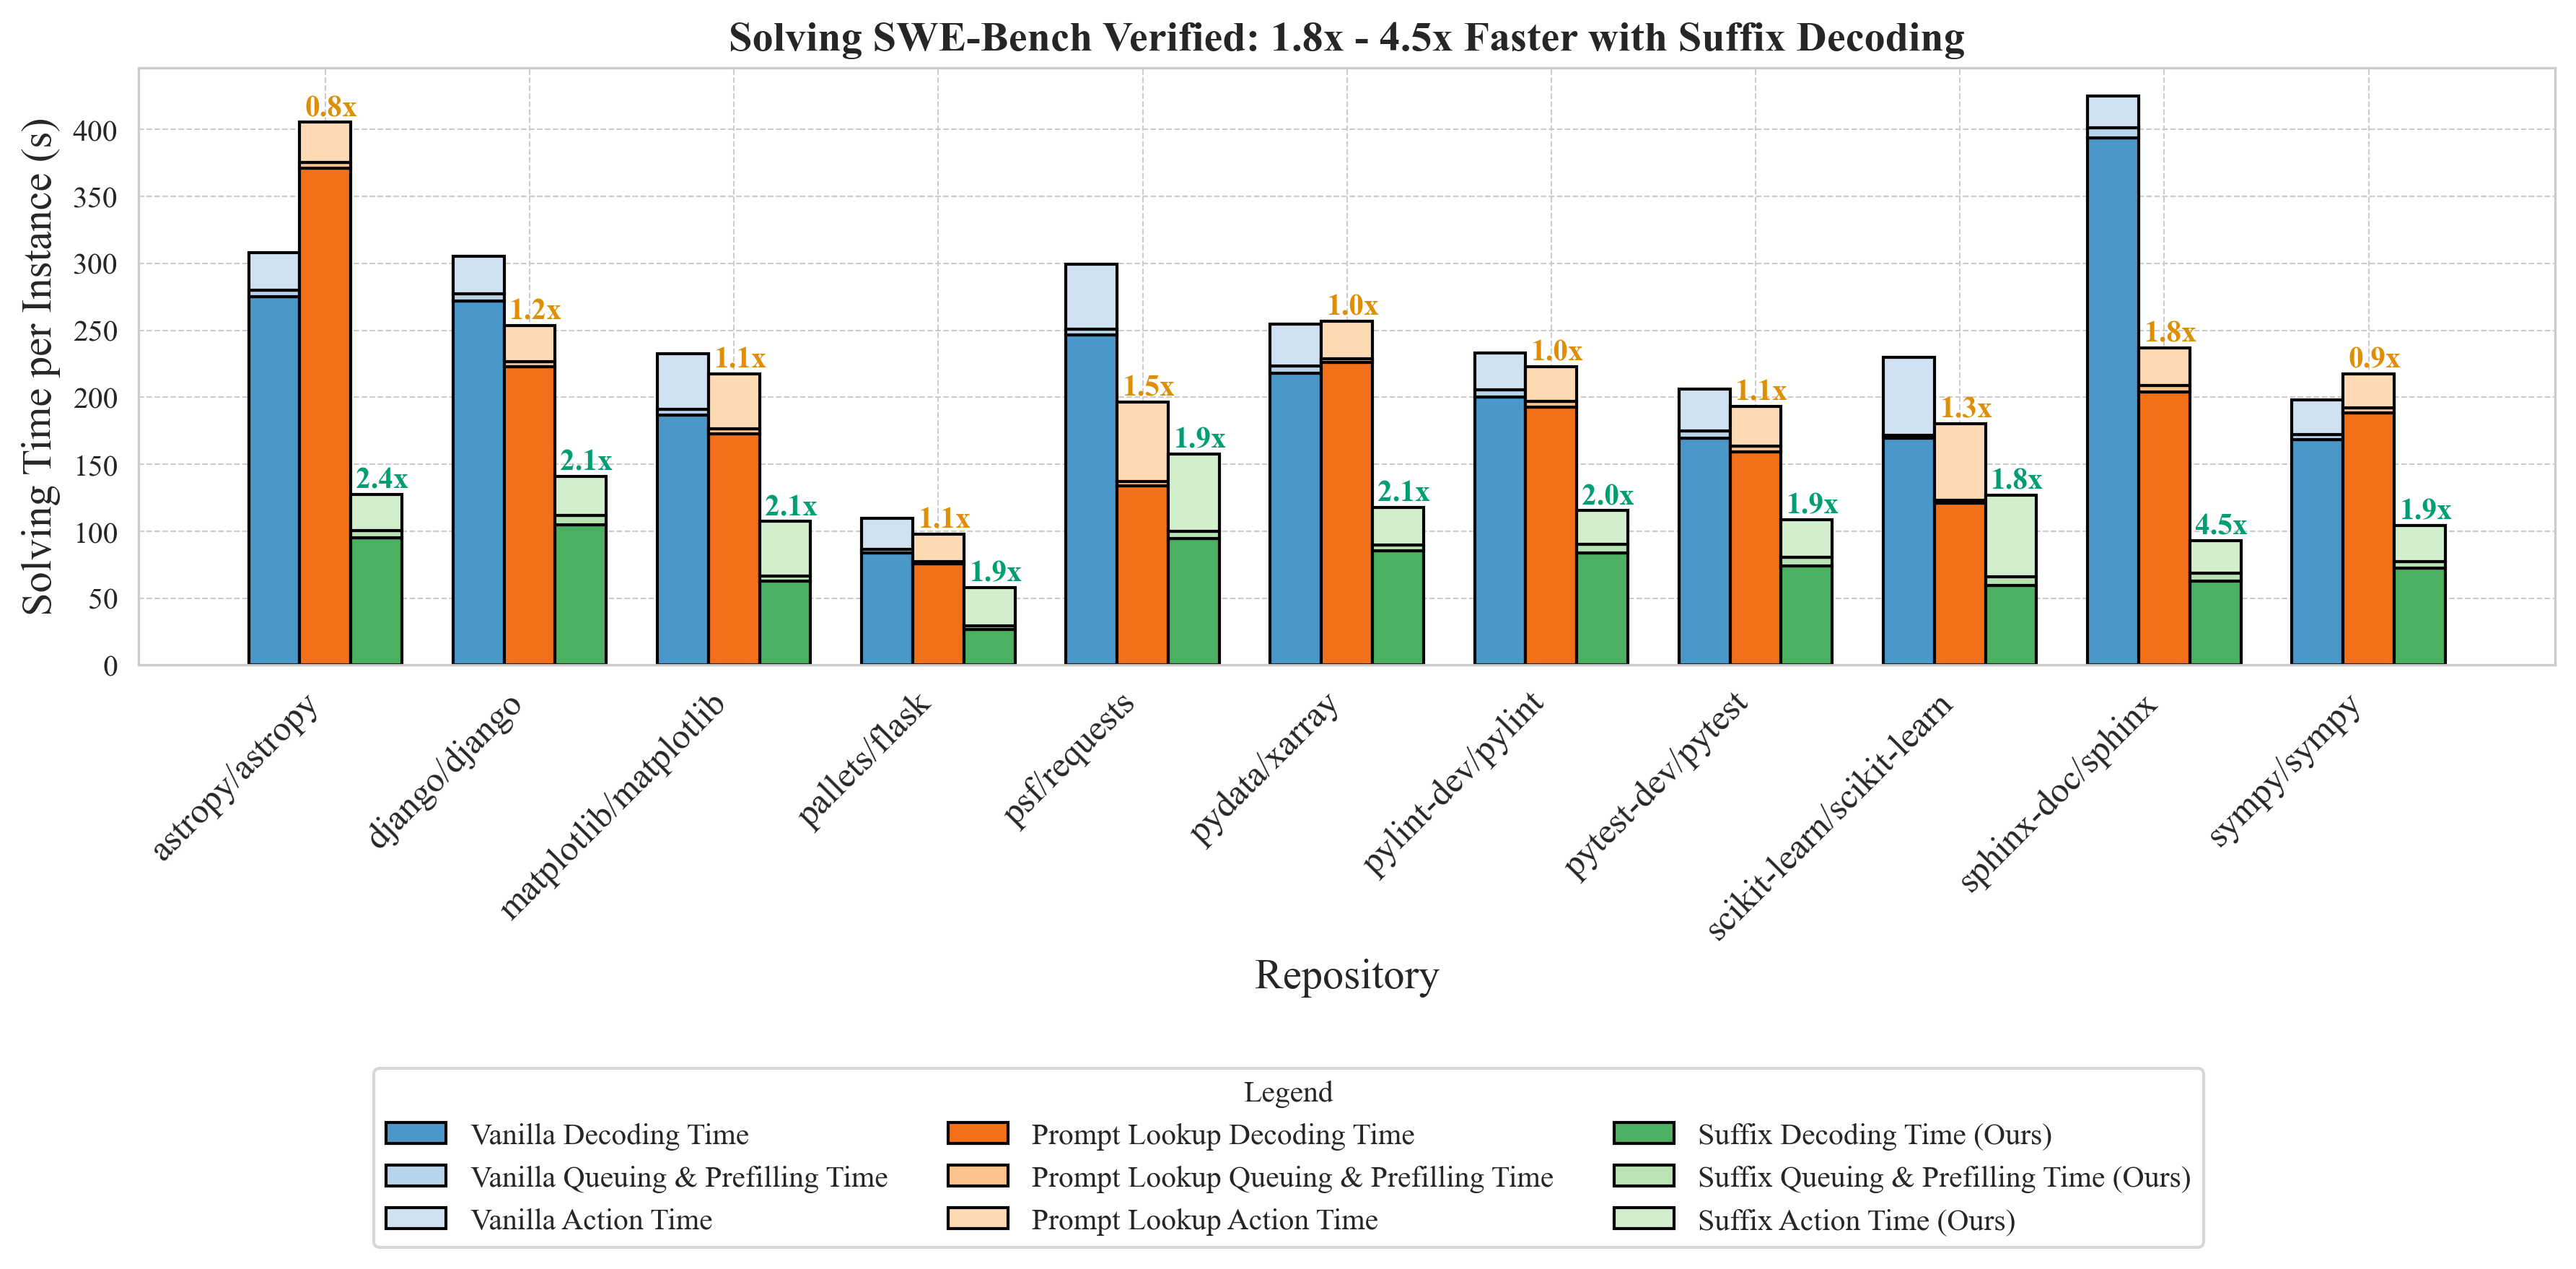
\includegraphics[width=\linewidth]{latex/figures/combined_latency_breakdown.png}
\caption{End-to-end task-completion time of the OpenHands agent on SWE-Bench Verified. The benchmarks are run with a concurrency of 8 tasks running simultaneously. vLLM is deployed on 4 H100 GPUs configured with 4-way tensor parallelism and prefix caching enabled. The results are broken down by the different code repositories in SWE-Bench.}
\label{fig:vllm-spec-bench}
\end{figure}

\subsection{Ablation Experiments}
\label{sec:ablation-experiments}

In this section, we present a few ablation studies on SuffixDecoding using a simulated verifier on offline traces. Given a ground-truth prompt-response pair from an LLM, we can verify the draft tokens proposed by SuffixDecoding by comparing with the ground truth responses. Additional ablation studies can be found in Appendix~\ref{sec:additional-ablation-experiments}.

\paragraph{Global vs per-request suffix trees.}

\begin{wrapfigure}{R}{0.5\textwidth}
    \centering
    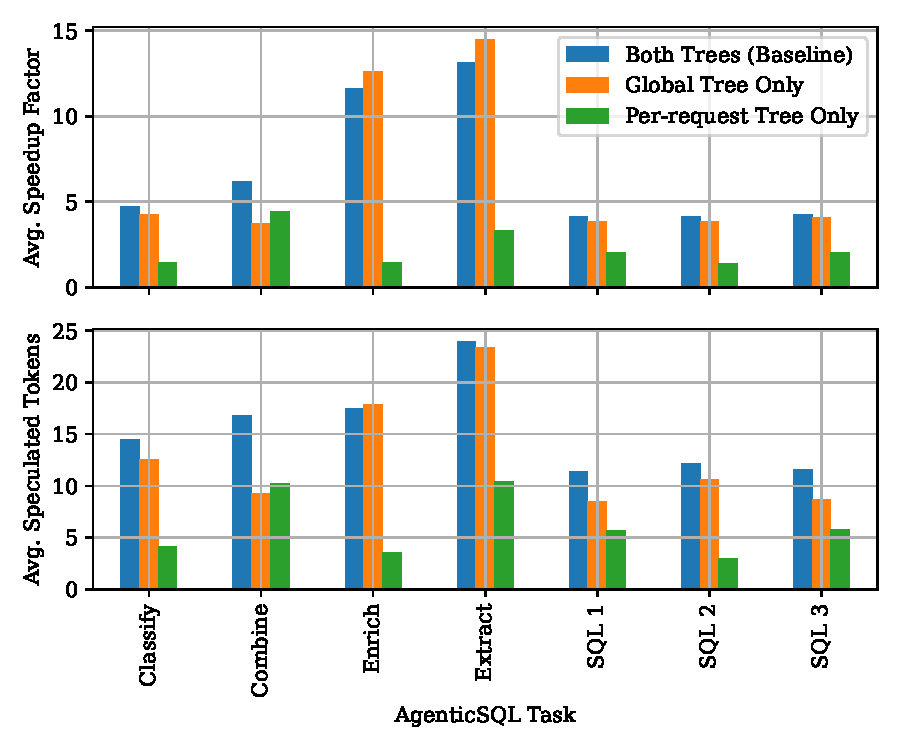
\includegraphics[width=0.5\columnwidth]{figures/per_request_tree.pdf}
    \caption{Speedup factor and number of speculated tokens for the tasks in AgenticSQL. SuffixDecoding was run with only the global suffix tree, only the per-request suffix tree, and both (baseline).}
    \label{fig:per-request-tree}
\end{wrapfigure}

We study the impact of the two suffix trees: the global suffix tree containing previous outputs, and the per-request suffix tree containing the prompt and generation of the current ongoing request. To do so, we ran the tasks in AgenticSQL using SuffixDecoding (1) with the global suffix tree only, (2) with the per-request suffix tree only, and (3) using both trees.

Fig.~\ref{fig:per-request-tree} shows the results. First, we note that with the exception of the Content Enrichment (Enrich) and Extract steps, using both suffix trees performs better than using just one. The small degradations on the enrich and extract steps suggest that, when both trees are present, SuffixDecoding may sometimes choose a speculation tree from the per-request suffix tree when the global suffix tree may have been the better choice. Improvements to SuffixDecoding's speculation tree scoring mechanism may help bridge this gap.

Second, the global tree outperforms the per-request tree on all tasks except for Combine. This is because the Combine task heavily re-uses tokens from its context, which are the proposed SQL solutions from the previous steps in the workflow. Although there is a diversity of task characteristics, SuffixDecoding is able to achieve high speedups on all of them by combining both suffix trees.

\paragraph{SuffixDecoding in open-ended scenarios.}

\begin{wrapfigure}{R}{0.5\textwidth}
\centering
\begin{subfigure}{0.25\columnwidth}
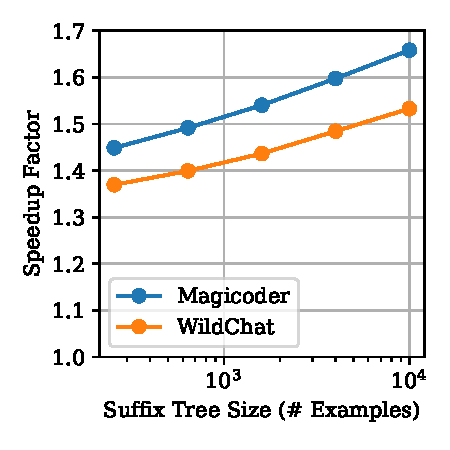
\includegraphics[width=\columnwidth,trim={5 5 5 5},clip]{figures/global_suffix_tree_size_speedup.pdf}
\end{subfigure}%
\hfill
\begin{subfigure}{0.25\columnwidth}
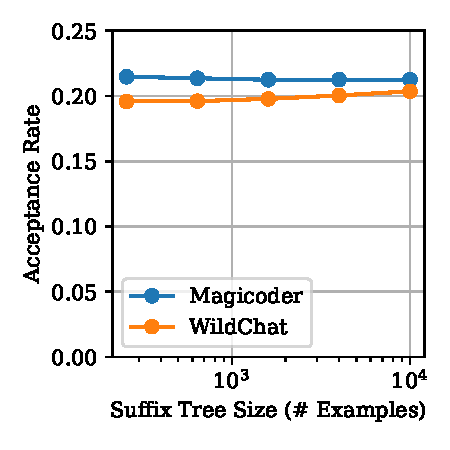
\includegraphics[width=\columnwidth,trim={5 5 5 5},clip]{figures/global_suffix_tree_size_acceptance.pdf}
\end{subfigure}
\caption{Speedup (left) and acceptance rate (right) vs global suffix tree size for Magicoder and Wildchat (\( \alpha = 1 \)). The speedup from SuffixDecoding continues to increase with more previous output examples, while the acceptance rate holds steady.}
\label{fig:global-suffix-tree-size}
\end{wrapfigure}

Although SuffixDecoding is designed for agentic workloads with long repeated token sequences, it is also interesting to evaluate it using more open-ended workloads like WildChat (open-ended chat)~\citep{zhao2024wildchat} and Magicoder (code-oriented chat)~\citep{wei2023magicoder}. Details on these datasets can be found in Appendix~\ref{sec:additional-ablation-experiments}.

In Fig.~\ref{fig:global-suffix-tree-size}, we show the speedup and acceptance rate of SuffixDecoding on WildChat and Magicoder across a range of suffix tree sizes between 256 and 10,000 output examples. First, we note a promising pattern: the speedup consistently improves as the size of the suffix tree grows. This indicates that SuffixDecoding can learn useful patterns even in workloads with lower token repetition, and may be a substitute for model-based methods when a draft model is not available.

Second, perhaps surprisingly, the acceptance rate does not change much even when the suffix tree size varies across almost two orders of magnitude. We believe this is primarily due to the effect of the adaptive speculation length \( \texttt{MAX\_SPEC} = \alpha p \). Although less data may mean less certainty in the speculated tokens, the pattern matches are also shorter, which results in fewer speculated tokens.